% PROGETTAZIONE 
\chapter{Progettazione e codifica }\label{chap:design}

\section {Progettazione architetturale e di dettaglio}
\subsection{Architettura OpenChat}
Avendo dovuto basare l'applicazione sulla soluzione già implementata per il web dalla \emph{zimlet OpenChat} è utile approfondire la sua \gl{architettura}{architettura} per comprendere le differenze applicate. \\
La comunicazione tra il server \emph{Zimbra} e la \emph{zimlet OpenChat} avviene attraverso una struttura \emph{\textbf{S}imple \textbf{O}bject \textbf{A}ccess \textbf{P}rotocol} (\acrshort{SOAP}), protocollo per lo scambio di messaggi tra componenti hardware.
Questa struttura, nel caso della \emph{zimlet OpenChat}, permette la comunicazione con il server indirettamente facendo passare gli eventi per il \emph{web client Zimbra} che li gestisce in base ai propri bisogni prima di inviarli al server. \\
\begin{figure}[H] 
	\centering
	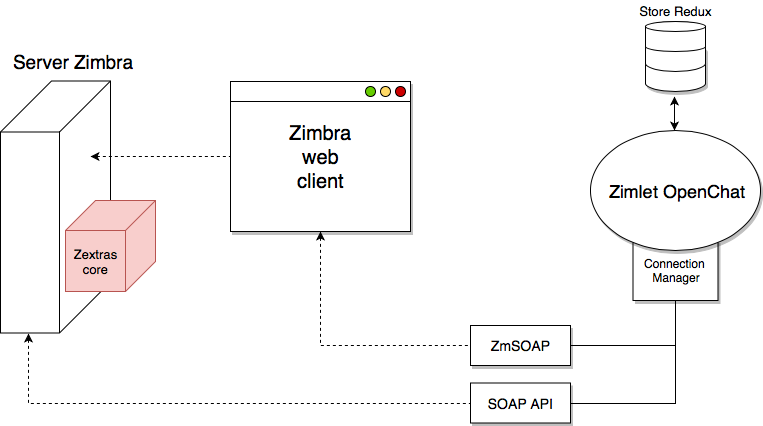
\includegraphics[scale=0.45]{architettura2}
	\caption{Architettura OpenChat}
\end{figure}
Dato che l'applicazione \emph{Teamwork} non interagisce con \emph{Zimbra web client} è stata modificata la modalità di ricezione ed invio dei messaggi SOAP e la gestione tramite \emph{connection manager} in modo da far comunicare direttamente \emph{Teamwork} e il server \emph{Zimbra} (con \emph{Zextras core} integrato).

\subsection{Gestione eventi}
Per gestire in modo ottimale ed efficacie la comunicazione tra server e client è stata strutturata un'architettura capace di reagire alla ricezione e all'invio di eventi. \\
Questa struttura permette la sincronizzazione dei dati tra il server e tutte le sessioni aperte facendo in modo di tenere aggiornato lo \emph{store} Redux di ogni applicazione connessa.\\
Di seguito un'approfondimento delle varie componenti che permettono questa interazione:
\begin{figure}[H] 
	\centering
	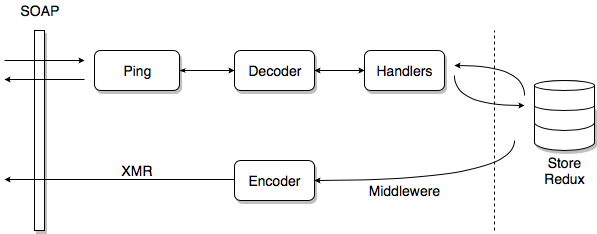
\includegraphics[scale=0.6]{architettura}
	\caption{Gestione eventi}
\end{figure}
\subsubsection{SOAP}
La trasmissione e la negoziazione dei messaggi scambiati tra server e client è regolata secondo i protocolli \emph{\textbf{H}yper\textbf{T}ext \textbf{T}ransfer \textbf{P}rotocol} (\acrshort{HTTP}) o \emph{\textbf{S}imple \textbf{M}ail \textbf{T}ransfer \textbf{P}rotocol}(\acrshort{SMTP}), all'interno dei quali viene incapsulato il messaggio SOAP.
I messaggi SOAP, rappresentati in figura \ref{fig:SOAP}, sono basati sul metalinguaggio \emph{e\textbf{X}tensible \textbf{M}arkup \textbf{L}anguage} (\acrshort{XML}) e vengono strutturati secondo due segmenti principali, \emph{head} e \emph{body}. 
\begin{figure}[H] 
	\centering
	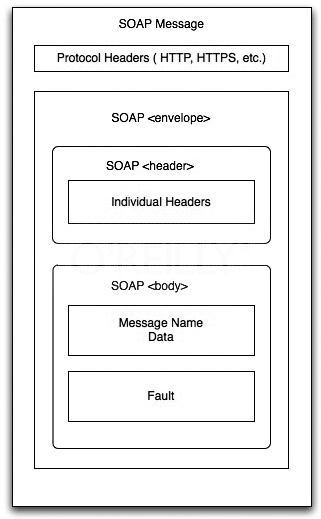
\includegraphics[scale=0.4]{SOAP}
	\caption{Struttura messaggio SOAP}
	\label{fig:SOAP}
\end{figure}
\begin{itemize}
	\item Il segmento \textbf{header} contiene metadati utili per la trasmissione del messaggio, come informazioni per il \emph{routing} e per la sicurezza. Può essere opzionale.
	\item Il segmento \textbf{body}, che invece risulta obbligatorio, trasporta il contenuto informativo (\emph{payload}) del messaggio. Saranno questi i dati importanti per la gestione delle informazioni.
\end{itemize}
Per ogni SOAP \emph{request} inviata al server ci sarà una SOAP \emph{respose} in ritorno. Questa risposta può contenere dati richiesti dalla precedente SOAP \emph{request}, informazioni sullo stato del server o possibili errori di risposta.
\subsubsection{Connection Manager}
È il \emph{connection manager} ad occuparsi degli eventi in arrivo dal server. Per fare ciò ha bisogno di due componenti principali:
\begin{itemize}
	\item il \textbf{ping}, componente che si occupa di stabilire una connessione con il server e di mantenerla operativa durante tutta la sessione. In questo modo l'applicazione rimarrà sempre in ascolto di nuovi eventi provenienti dal server;
	\item il \textbf{decoder}, componente che, una volta ricevuto un messaggio SOAP dal \emph{ping}, ne decodificherà il \emph{body} permettendo una più facile comprensione del contenuto. Si è utilizzato un \emph{Abstract Factory} per la creazione di questa componente, \gl{design pattern}{design pattern} che fornisce un’interfaccia per creare famiglie di prodotti senza specificare classi concrete.
\end{itemize}
\subsubsection{Handlers}
Questa famiglia di componenti riceve in input degli eventi provenienti dal \emph{decoder}. Questo vuol dire che non riceve dei generici messaggi SOAP ma dei \emph{\textbf{J}avaScript \textbf{O}bject \textbf{N}otation}(\acrshort{JSON}) associati a dei particolari eventi di cui è stato implementato un \textbf{handler} specifico.\\
La sua funzione, quindi, è quella di modificare lo stato dello \emph{store} Redux, basandosi sui dati ricevuti, attraverso un \emph{dispatcher} che modifica il flusso dei dati utilizzati nell'applicazione in modo unidirezionale, così da non creare inconsistenza.
\subsubsection{Encoder}
Gli eventi possono essere generati anche dall'applicazione e per gestire il bisogno di propagare le modifiche che vengono fatte allo \emph{store} Redux al server (con la successiva propagazione dei dati verso le altre sessioni) è stato introdotto un \textbf{encoder}, il corrispondente del precedente componente \emph{decoder} per l'invio degli eventi. \\
Quando viene fatto il \emph{dispatch} di un'azione con la conseguente modifica dello \emph{store} vengono invocati dei particolari \emph{middleware} che si occupano dell'invio dell'evento all'\emph{encoder} corrispondente. Questa componente permette la traduzione dell'evento in un messaggio SOAP generico comprensibile dal server.

\subsection{Store Redux}
L'architettura disegnata per la gestione degli eventi ha come punto focale il concetto di \emph{store}, \emph{database} locale dove vengono salvati tutti i dati necessari all'implementazione tramite React Native dell'interfaccia grafica. Come è stato spiegato nel capitolo \emph{Tecnologie utilizzate} (\ref{subsec:Redux}) uno \emph{store} Redux è un \emph{database} dinamico condiviso, accessibile da tutte le componenti di React Native così che possano sempre avere dei dati coerenti tra loro. \\
Tramite il design pattern architetturale implementato da Redux, Flux, è stato possibile ottimizzare la gestione dei dati in modo reattivo all'arrivo degli eventi. \\
In particolare è stato deciso di introdurre due \emph{store} distinti nell'applicazione:
\begin{itemize}
	\item lo \textbf{Store OpenChat }è stato ereditato dall'implementazione della \emph{zimlet OpenChat} in quanto, per ottenere dei dati sincronizzati, deve necessariamente rispecchiare la sua struttura. Questo \emph{store} è quindi connesso alla gestione degli eventi tramite il \emph{connection manager} ed è la fonte principale dei dati funzionali per l'applicazione.
	\item lo \textbf{Store Teamwork}, invece, detiene dati operativi utili alla gestione dell'applicazione e importanti per mantenere la sessione attiva.
\end{itemize} 
\subsubsection{Diagramma delle classi store Redux Teamwork}
\begin{figure}[H] 
	\centering
	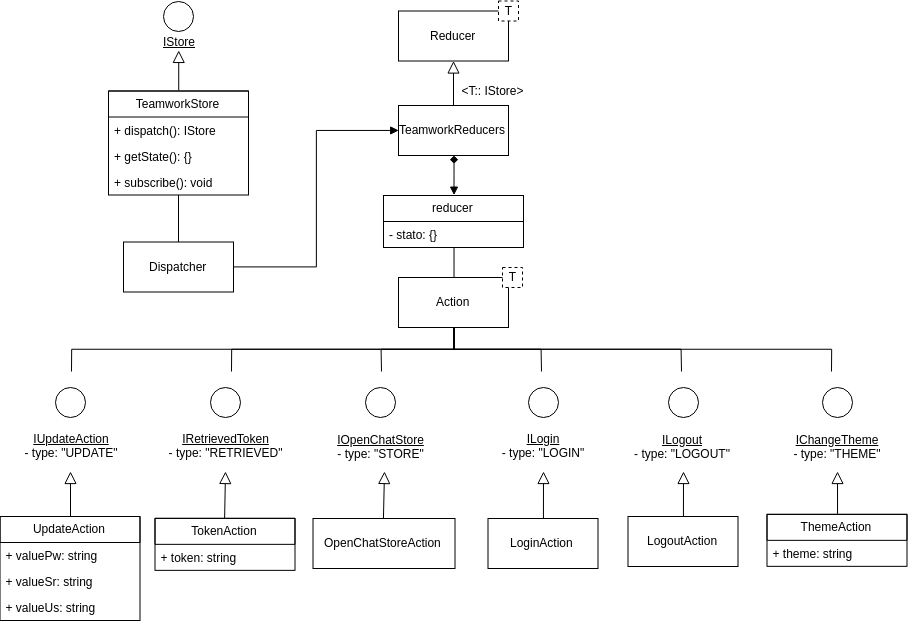
\includegraphics[scale=0.45]{TeamworkStore}
	\caption{Redux store utilizzato per gestire Teamwork}
\end{figure}

\section{Progettazione grafica}
Prima di procedere alla definizione delle classi necessarie per l'implementazione 
dell'applicazione è stato deciso di effettuare la progettazione della \emph{\textbf{U}ser \textbf{I}nterface} (\acrshort{UI}) per far 
si che il progetto di stage abbracciasse a 360 gradi il processo di sviluppo di 
un'applicazione da parte di un'azienda.

\subsection{Wireframe}
In base ai requisiti e agli use case raccolti è stato definito il modello iniziale
 dell'applicazione tramite la realizzazione dei \textbf{wireframe} delle varie schermate. \\
Questo studio è la prima rappresentazione visuale dell'applicazione ed ha lo 
scopo di identificare la struttura, l'architettura dell'informazione e la 
disposizione degli elementi nella pagina.\\
Di seguito vengono riportati i \emph{wireframe} sviluppati di alcune delle pagine più 
importanti di \emph{Teamwork}:
\begin{figure}[H] 
	\centering
	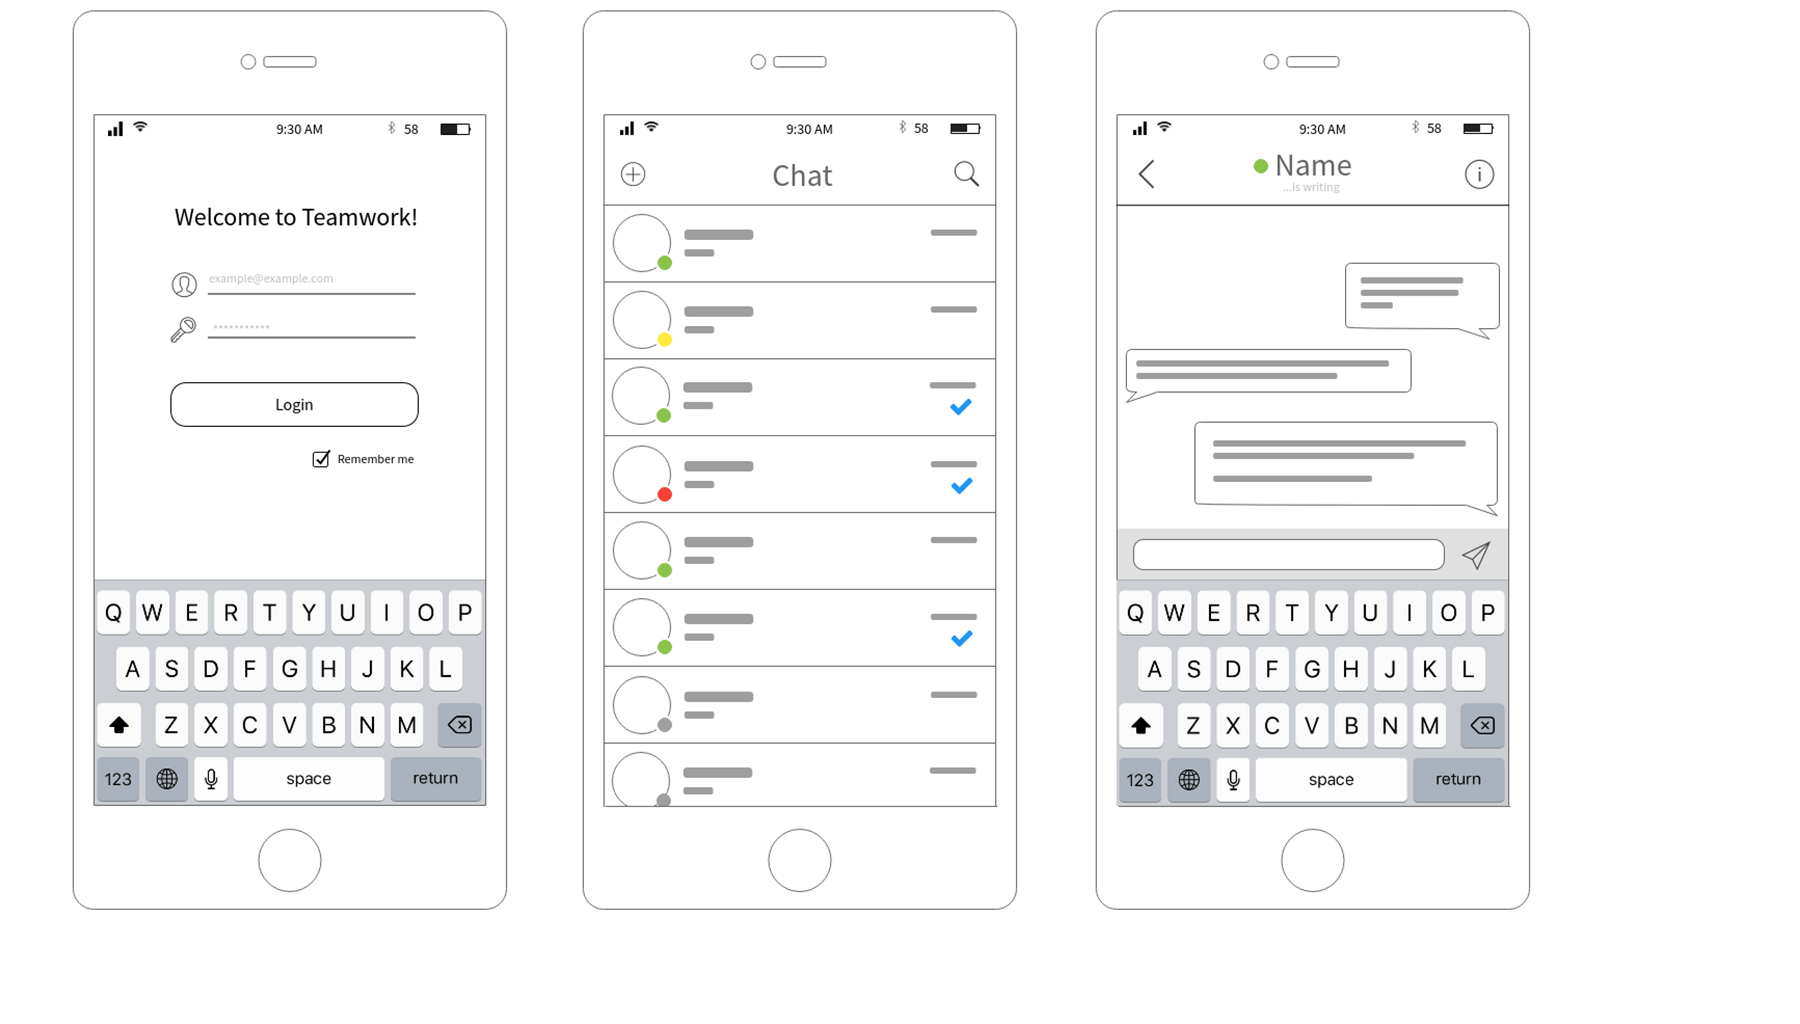
\includegraphics[scale=0.5]{wireframe}
	\caption{Wireframe pagina di login, buddylist e chat page.}
	\label{subsec:wireframe}
\end{figure}
Come possiamo notare dagli esempi riportati, in questa fase non è stato deciso 
nulla riguardo la rappresentazione grafica dei vari elementi. 
Si è definita soltanto la struttura delle varie schermate, il collegamento tra 
di esse e quali elementi realmente soddisfino i requisiti già studiati. 
Il risultato, comunque, è stato molto vicino alla \emph{\textbf{G}raphical \textbf{U}ser \textbf{I}nterface} (\acrshort{GUI}) ottenuta alla fine della 
codifica in quando i \emph{wireframe} sono stati disegnati tenendo conto della 
soluzione web già presente.\\ 
Questo passo è stato essenziale per rendere più chiara l'idea del prodotto desiderato.

\subsection{Linee guida}
Per quanto riguarda la GUI vera e propria sono state fornite dall'azienda delle 
\emph{guidelines} da seguire per la rappresentazione grafica di ogni elemento. \\
Nello specifico le \emph{guidelines} toccano temi come:
\begin{itemize}
	\item le proporzioni tra i componenti;
	\item i colori da utilizzare;
	\item le definizioni di alcuni elementi base;
\end{itemize}
Questo serve per avere uno stile comune tra le varie applicazioni che 
l'azienda sviluppa. \\
Un esempio è la definizione del componente \emph{card}, destinato alla 
visualizzazione dei dettagli relativi ad un \emph{buddy}:
\begin{figure}[H] 
	\centering
	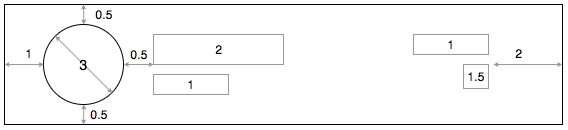
\includegraphics[scale=0.5]{guidelines}
	\caption{Esempio guidelines spazi}
\end{figure}
Si noti come ogni elemento sia posizionato in modo preciso definendo delle 
proporzioni tra gli spazi. In questo modo la successiva codifica dello stile sarà 
assolutamente definita da regole precise in modo da non dover interagire in modo 
continuativo con il responsabile grafico del progetto. \\
L'applicazione delle \emph{guidelines} nel codice è avvenuta in parallelo con lo sviluppo 
in quando, seguendo una metodologia \emph{agile}, si è ritenuto opportuno che le varie 
versioni prototipali dell'applicazione avessero anche una progressiva applicazione 
delle regole di stile.\\
Approvati i \emph{wireframe} è stato possibile proseguire alla definizione di tutti 
e soli i componenti veramente utili al \emph{layout}.

\section{Interfaccia grafica con React Native}
Per la realizzazione della UI è stato utilizzato il \emph{framework} React Native che consente la realizzazione di interfacce tramite la suddivisione del sistema in componenti. Ognuna di queste ha un proprio stato, delle proprietà che vengono ereditate dal componente padre, e un proprio ciclo di vita indipendente da qualsiasi altro.
\newline
Sono stati progettati i componenti e la gerarchia tra essi necessaria per la visualizzazione degli \emph{screen} precedentemente definiti e realizzata una navigazione tra le pagine in modo da rispettare la gerarchia.
\begin{figure}[H] 
	\centering
	
\includegraphics[scale=0.7]{boh}
	\caption{Relazione tra screen}
	\label{gerarchiaRN}
\end{figure}
L'immagine \ref{gerarchiaRN} descrive le relazioni tra le componenti implementate.
\note{Spiegare l'immagine quando ce l'avrò}
